\documentclass{beamer}
\usetheme{Warsaw}
 \usecolortheme{crane}
\usepackage{lmodern}
\usepackage[utf8]{inputenc}
\setbeamertemplate{navigation symbols}{}
\usepackage{listings}

\title[\insertframenumber/\inserttotalframenumber]
      {Research paper presentation:\\
       ``De-indirection for Flash-based SSDs with Nameless Writes''\\
       \small{Y. Zhang, L. P. Arulraj, A. C. Arpaci-Dusseau, R. H. Arpaci-Dusseau}}
\author{Federico Wasserman \& Rodolphe Lepigre}
\institute{MOSIG - Parallel, Distributed and Embedded Systems}

\AtBeginSection[]{
  \begin{frame}
    \small \tableofcontents[currentsection, hideothersubsections]
  \end{frame} 
}

\begin{document}

\begin{frame}
\titlepage
\end{frame}

\begin{frame}
  \frametitle{Outline}
  \tableofcontents[hideallsubsections]
\end{frame}

\section{Introduction}
\begin{frame}
  \frametitle{What are Nameless Writes?}
  \begin{itemize}
    \item New device interface for SSDs
    \item Remove the need for indirection
    \item Idea: the device chooses WHERE to write
  \end{itemize}
\end{frame}

\begin{frame}
  \frametitle{How are Nameless Writes different?}
  Usual Writes:
  \begin{itemize}
    \item The FS requests the writing of data at some location
    \item The device performs the write
  \end{itemize}

  Nameless Writes:
  \begin{itemize}
    \item The FS requests the writing of data
    \item The device performs the write
    \item Address returned to the FS
  \end{itemize}
\end{frame}

\section{SSD principles}
\begin{frame}
% TODO
\end{frame}

\section{Indirection in SSDs}
\begin{frame}
  \frametitle{SSDs need indirection}
  \begin{itemize}
    \item Indirection is used to implement wear-leveling
    \item Absolutely necessary to ensure reasonable lifetime
    \item Problem: need to store indirection table
    \item 3 main techniques:
          \begin{itemize}
            \item Full-page mapping
            \item Block mapping
            \item Hybrid mapping
          \end{itemize}
  \end{itemize}
\end{frame}

\begin{frame}
  \frametitle{Full-page mapping}
  \begin{itemize}
    \item Each page can be mapped
    \item Consider 32-bit pointers per 2KB pages
    \item With 1TB SSD, 2GB indirection table
    \item Problem: Great space overhead, DRAM is expensive
  \end{itemize}
\end{frame}

\begin{frame}
  \frametitle{Block mapping}
  \begin{itemize}
    \item Mapping at block-level (128 pages)
    \item 32MB indirection table in the same settings
    \item Smaller memory overhead
    \item Problem: high garbage collection cost (Gupta et al.)
  \end{itemize}
\end{frame}

\begin{frame}
  \frametitle{Hybrid mapping}
  \begin{itemize}
    \item Map most data at block level
    \item Small page-mapped area
    \item Keeps space overhead low
    \item Avoids garbage collection overhead
    \item Problem: garbage collection can still hurt performances
    \item Problem: very complex FTL (Flash Translation Layer)
    \item Solution: Nameless Writes
  \end{itemize}
\end{frame}

\section{Nameless Writes}
\begin{frame}
  \frametitle{Reminder}
  Idea: the device chooses WHERE to write
  \begin{itemize}
    \item The FS requests the writing of data
    \item The device performs the write
    \item Address returned to the FS
  \end{itemize}
\end{frame}

\begin{frame}[fragile]
  \frametitle{Main interface}
  \begin{lstlisting}
Nameless_Write(data, len) : phys@
Nameless_Overwrite(phys@, data, len) : new@
Physical_Read(phys@, len) : data
Free(vitr/phys@, len)
  \end{lstlisting}
\end{frame}

\begin{frame}
  \frametitle{Recursive update problem}
  \begin{itemize}
    \item Problem with this interface: recursive update
    \item File modification imply inode update
    \item The inode will move (Nameless overwrite)
    \item Every structure pointing to it will have to be updated
    \item ...
  \end{itemize}
\end{frame}

\begin{frame}
  \frametitle{Inode, and file structure}
  \begin{center}
  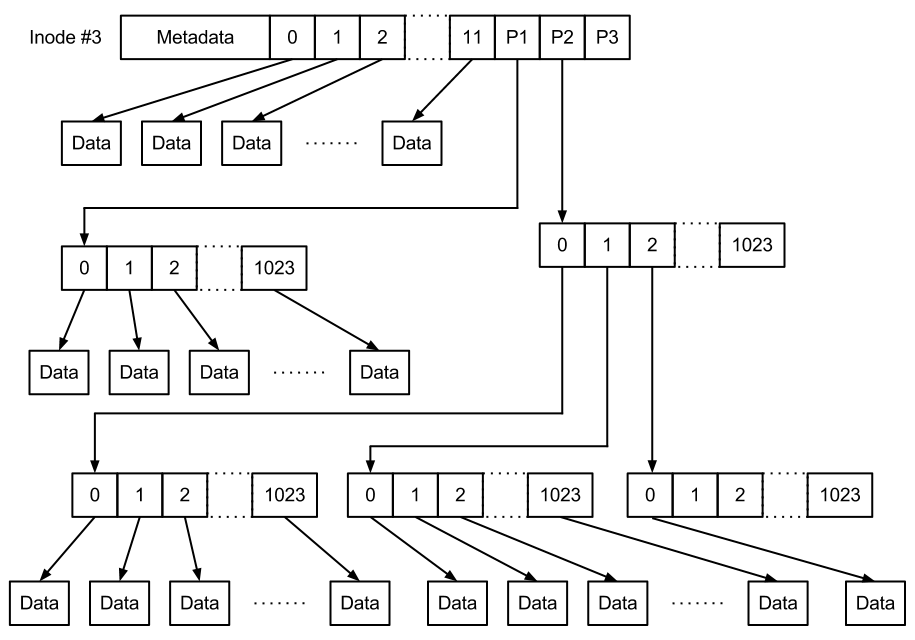
\includegraphics[width=250px]{inode.png}
  \end{center}
\end{frame}

\begin{frame}
  \frametitle{File tree}
  \begin{center}
  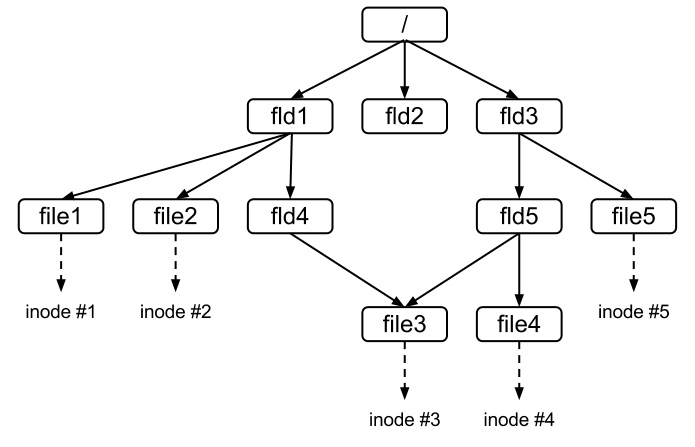
\includegraphics[width=250px]{file_tree.png}
  \end{center}
\end{frame}

\begin{frame}
  \frametitle{Solution: Segmented address space}
  \begin{itemize}
    \item Large physical address space (for nameless writes)
    \item Small virtual address space (for traditional writes)
    \item Idea: keep pointer-based structures in virtual space
  \end{itemize}
\end{frame}

\begin{frame}
  \frametitle{Segmented address space}
  \begin{center}
  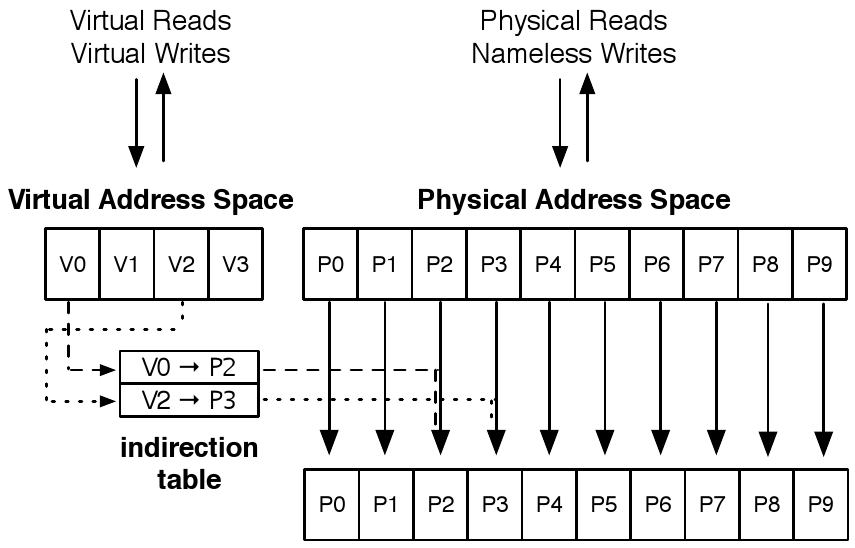
\includegraphics[width=250px]{segmented.png}
  \end{center}
\end{frame}

\begin{frame}[fragile]
  \frametitle{Virtual read / write interface}
  \begin{lstlisting}
Virtual_Write(virt@, data, len)
Virtual_Read(virt@, len) : data
  \end{lstlisting}
\end{frame}

\begin{frame}[fragile]
  \frametitle{Migration callback}
  \begin{itemize}
    \item Callback provided for the SSD to notice data migration to the FS
    \item Useful for it to reclaim blocks (garbage collection)
  \end{itemize}
  \begin{lstlisting}
Migration [Callback] (old_phys@, new_phys@)
  \end{lstlisting}
\end{frame}

\section{Evaluation}
\begin{frame}
% TODO
\end{frame}

\section{Conclusion}
\begin{frame}
% TODO
\end{frame}

\end{document}

